\providecommand{\main}{../../main}
\documentclass[../main.tex]{subfiles}

\let\cleardoublepage\clearpage

\begin{document}
\appendix

\chapter{Models}
\label{sec:App_Model}
Here the variable distributions for the three different datasets are presented. Both leptonic channels are shown.

\section{Input data set - electron channel -}
\begin{figure}[!ht] 
  \begin{minipage}[b]{0.33\linewidth}
    \centering
    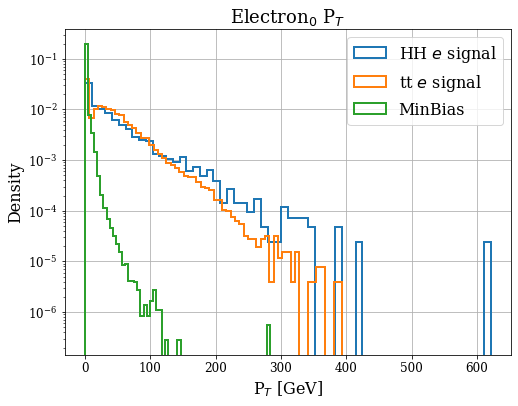
\includegraphics[width=1\linewidth]{Chapters/Plots/Hist_1ele_electron0_Et.png}
    %\vspace{4ex}
  \end{minipage}%%
  \begin{minipage}[b]{0.33\linewidth}
    \centering
    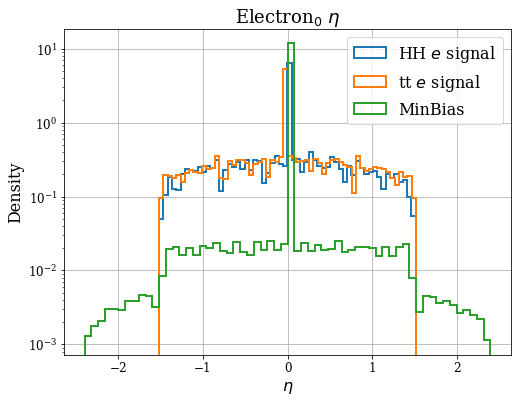
\includegraphics[width=1\linewidth]{Chapters/Plots/Hist_1ele_electron0_Eta.png}
    %\vspace{4ex}
  \end{minipage} %%
  \begin{minipage}[b]{0.33\linewidth}
    \centering
    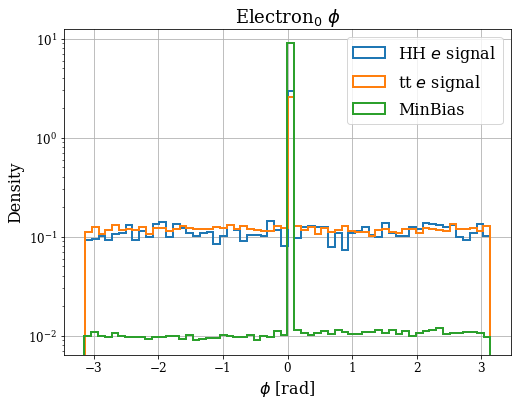
\includegraphics[width=1\linewidth]{Chapters/Plots/Hist_1ele_electron0_Phi.png}
    %\vspace{4ex}
  \end{minipage}
  \caption{Electron 0 variables}
\end{figure}

\begin{figure}[!ht] 
  \begin{minipage}[b]{0.33\linewidth}
    \centering
    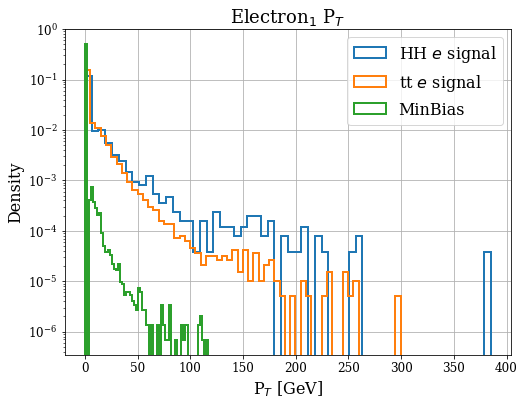
\includegraphics[width=1\linewidth]{Chapters/Plots/Hist_1ele_electron1_Et.png}
    %\vspace{4ex}
  \end{minipage}%%
  \begin{minipage}[b]{0.33\linewidth}
    \centering
    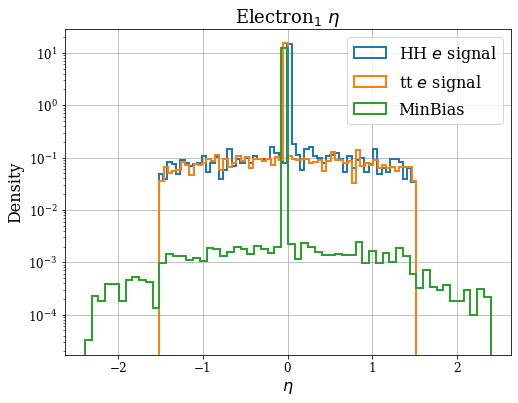
\includegraphics[width=1\linewidth]{Chapters/Plots/Hist_1ele_electron1_Eta.png}
    %\vspace{4ex}
  \end{minipage} %%
  \begin{minipage}[b]{0.33\linewidth}
    \centering
    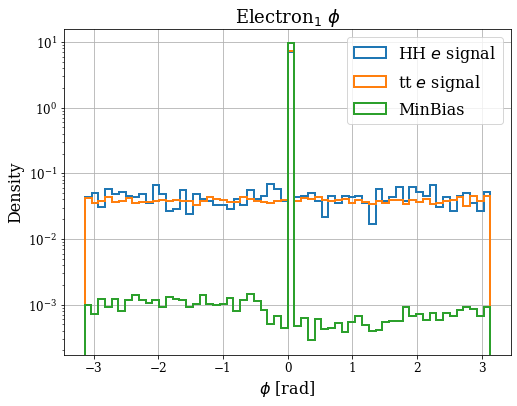
\includegraphics[width=1\linewidth]{Chapters/Plots/Hist_1ele_electron1_Phi.png}
    %\vspace{4ex}
  \end{minipage}
  \caption{Electron 1 variables}
 \end{figure}
 
 \begin{figure}[!ht]
  \begin{minipage}[b]{0.33\linewidth}
    \centering
    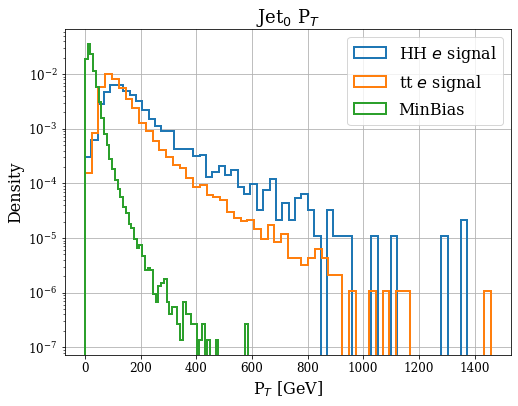
\includegraphics[width=1\linewidth]{Chapters/Plots/Hist_1ele_jet0_Et.png}
    %\vspace{4ex}
  \end{minipage}%%
  \begin{minipage}[b]{0.33\linewidth}
    \centering
    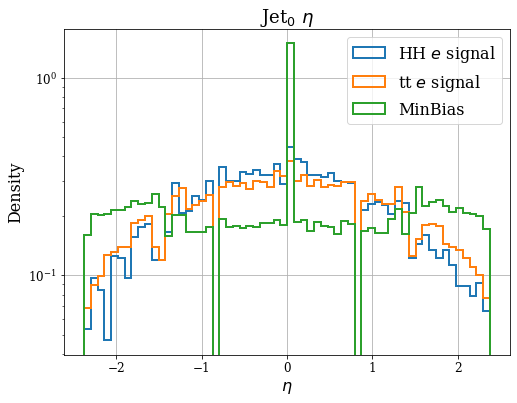
\includegraphics[width=1\linewidth]{Chapters/Plots/Hist_1ele_jet0_Eta.png}
    %\vspace{4ex}
  \end{minipage} %%
  \begin{minipage}[b]{0.33\linewidth}
    \centering
    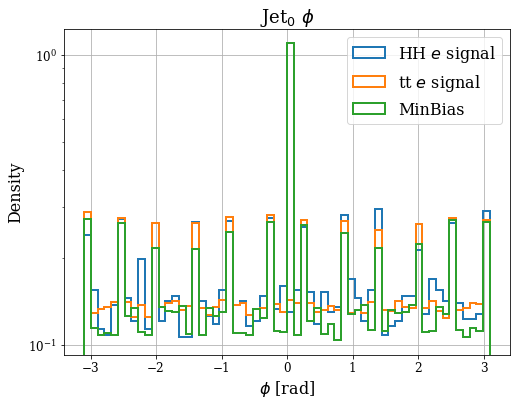
\includegraphics[width=1\linewidth]{Chapters/Plots/Hist_1ele_jet0_Phi.png}
    %\vspace{4ex}
  \end{minipage}
  \caption{Jet 0 variables}
 \end{figure}
 
 \begin{figure}[!ht]
  \begin{minipage}[b]{0.33\linewidth}
    \centering
    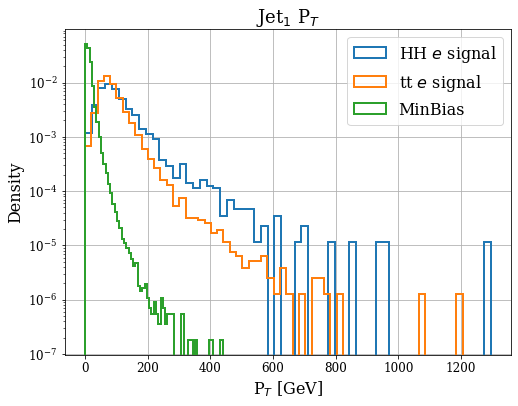
\includegraphics[width=1\linewidth]{Chapters/Plots/Hist_1ele_jet1_Et.png}
    %%%\vspace{4ex}
  \end{minipage}%%
  \begin{minipage}[b]{0.33\linewidth}
    \centering
    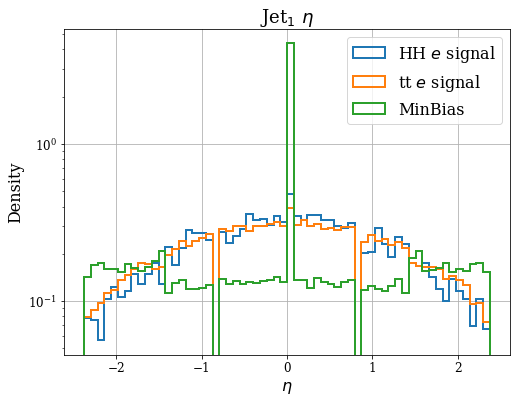
\includegraphics[width=1\linewidth]{Chapters/Plots/Hist_1ele_jet1_Eta.png}
    %%%\vspace{4ex}
  \end{minipage} %%
  \begin{minipage}[b]{0.33\linewidth}
    \centering
    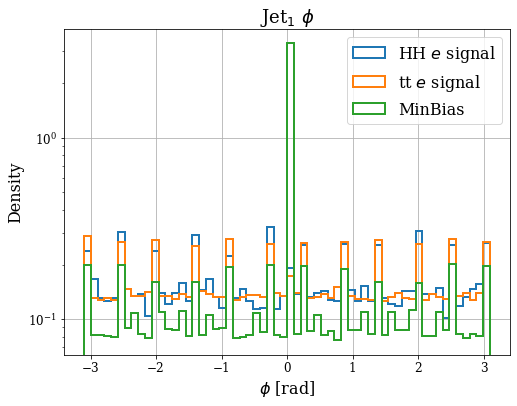
\includegraphics[width=1\linewidth]{Chapters/Plots/Hist_1ele_jet1_Phi.png}
    %%%\vspace{4ex}
  \end{minipage}
  \caption{Jet 1 variables}
 \end{figure}
 
 \begin{figure}[!ht]
  \begin{minipage}[b]{0.33\linewidth}
    \centering
    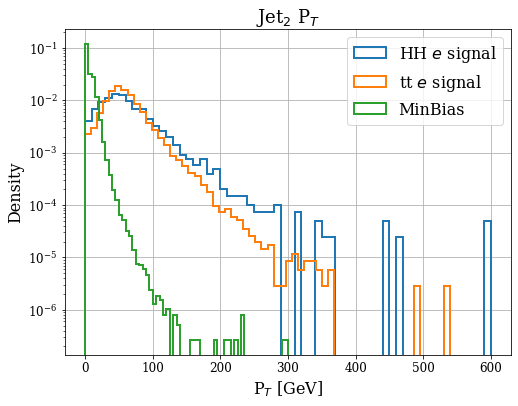
\includegraphics[width=1\linewidth]{Chapters/Plots/Hist_1ele_jet2_Et.png}
    %%%\vspace{4ex}
  \end{minipage}%%
  \begin{minipage}[b]{0.33\linewidth}
    \centering
    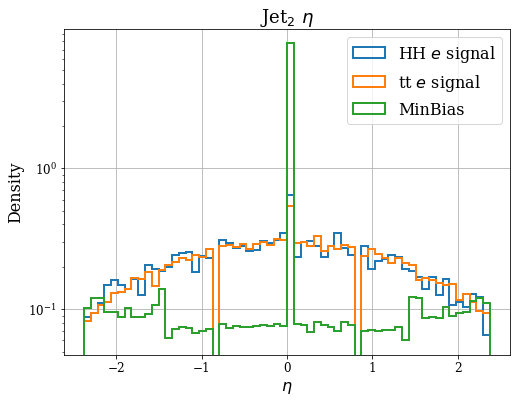
\includegraphics[width=1\linewidth]{Chapters/Plots/Hist_1ele_jet2_Eta.png}
    %%%\vspace{4ex}
  \end{minipage} %%
  \begin{minipage}[b]{0.33\linewidth}
    \centering
    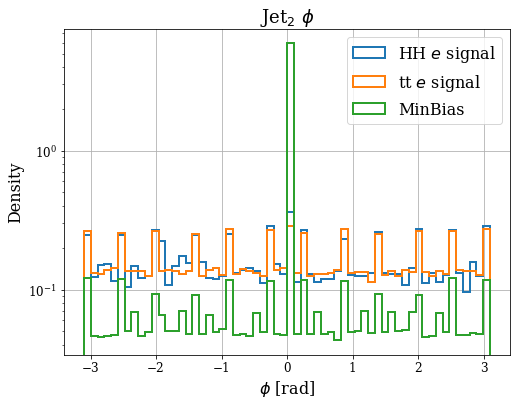
\includegraphics[width=1\linewidth]{Chapters/Plots/Hist_1ele_jet2_Phi.png}
    %%%\vspace{4ex}
  \end{minipage}
  \caption{Jet 2 variables}
\end{figure}

\begin{figure}[!ht]
  \begin{minipage}[b]{0.33\linewidth}
    \centering
    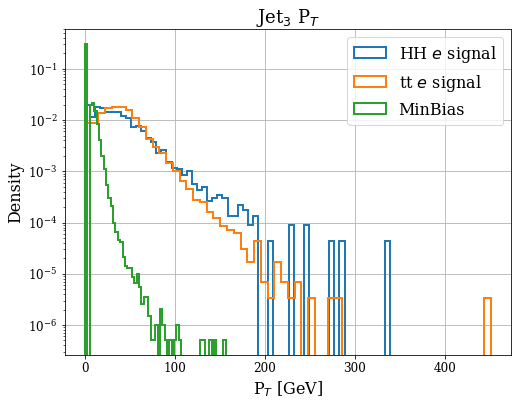
\includegraphics[width=1\linewidth]{Chapters/Plots/Hist_1ele_jet3_Et.png}
    %%%\vspace{4ex}
  \end{minipage}%%
  \begin{minipage}[b]{0.33\linewidth}
    \centering
    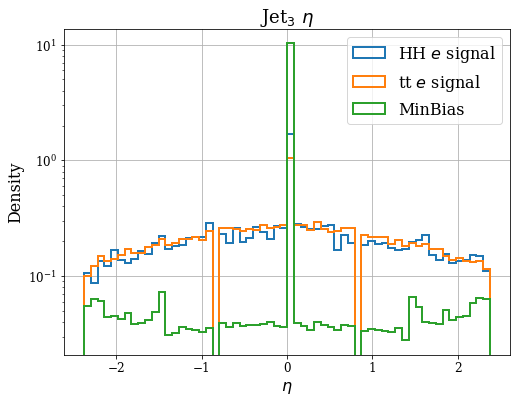
\includegraphics[width=1\linewidth]{Chapters/Plots/Hist_1ele_jet3_Eta.png}
    %%%\vspace{4ex}
  \end{minipage} %%
  \begin{minipage}[b]{0.33\linewidth}
    \centering
    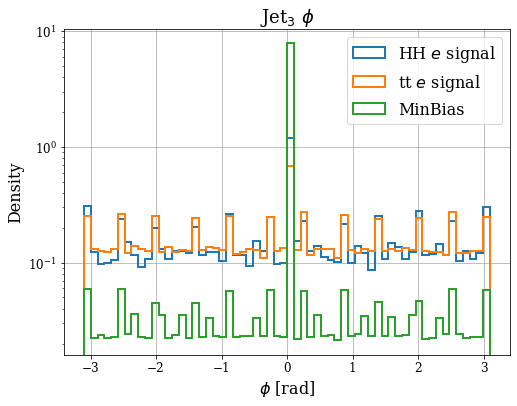
\includegraphics[width=1\linewidth]{Chapters/Plots/Hist_1ele_jet3_Phi.png}
    %%%\vspace{4ex}
  \end{minipage}
  \caption{Jet 3 variables}
\end{figure}

\begin{figure}[!ht]
  \begin{minipage}[b]{0.33\linewidth}
    \centering
    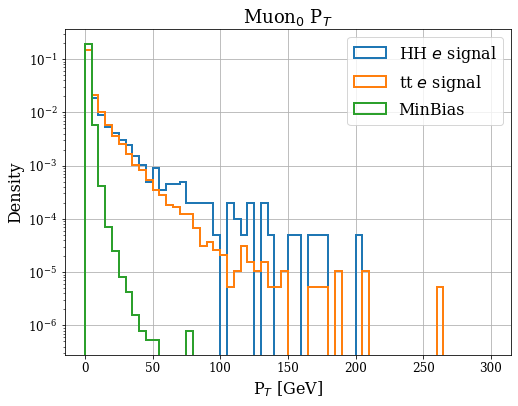
\includegraphics[width=1\linewidth]{Chapters/Plots/Hist_1ele_muon0_Pt.png}
    %%%\vspace{4ex}
  \end{minipage}%%
  \begin{minipage}[b]{0.33\linewidth}
    \centering
    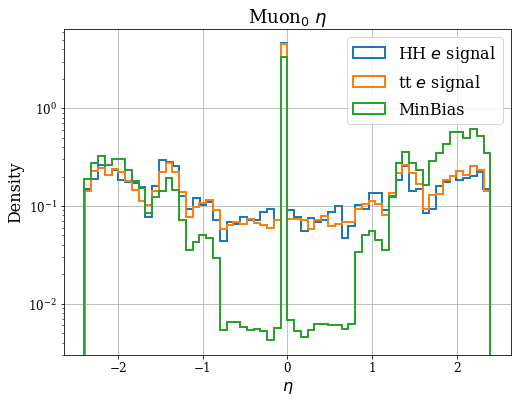
\includegraphics[width=1\linewidth]{Chapters/Plots/Hist_1ele_muon0_Eta.png}
    %%\vspace{4ex}
  \end{minipage} %%
  \begin{minipage}[b]{0.33\linewidth}
    \centering
    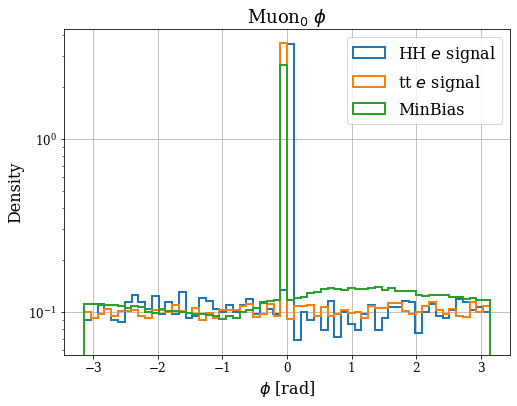
\includegraphics[width=1\linewidth]{Chapters/Plots/Hist_1ele_muon0_Phi.png}
    %%\vspace{4ex}
  \end{minipage}
  \caption{Muon 0 variables}
\end{figure}

\begin{figure}[!ht]
  \begin{minipage}[b]{0.33\linewidth}
    \centering
    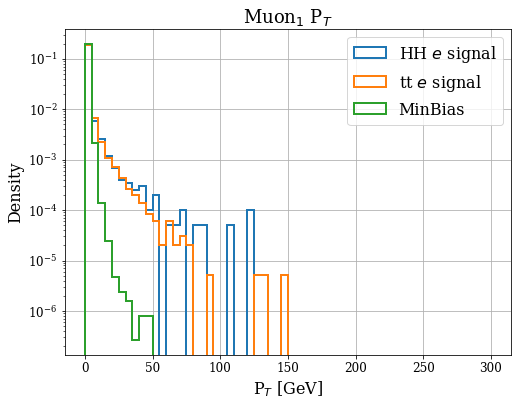
\includegraphics[width=1\linewidth]{Chapters/Plots/Hist_1ele_muon1_Pt.png}
    %%\vspace{4ex}
  \end{minipage}%%
  \begin{minipage}[b]{0.33\linewidth}
    \centering
    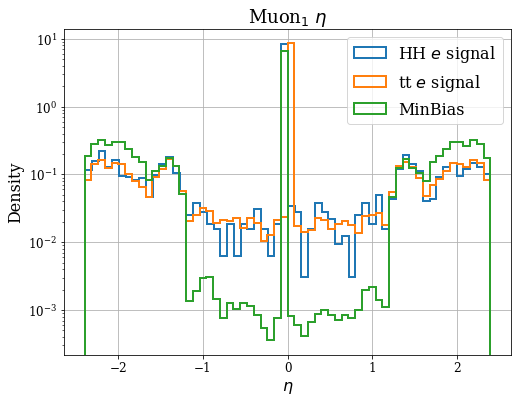
\includegraphics[width=1\linewidth]{Chapters/Plots/Hist_1ele_muon1_Eta.png}
    %\vspace{4ex}
  \end{minipage} %%
  \begin{minipage}[b]{0.33\linewidth}
    \centering
    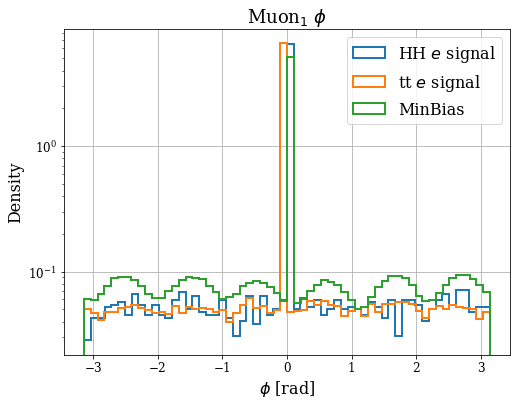
\includegraphics[width=1\linewidth]{Chapters/Plots/Hist_1ele_muon1_Phi.png}
    %\vspace{4ex}
  \end{minipage}
  \caption{Muon 1 variables}
\end{figure}

\begin{figure}[t]
  \begin{minipage}[b]{0.5\linewidth}
    \centering
    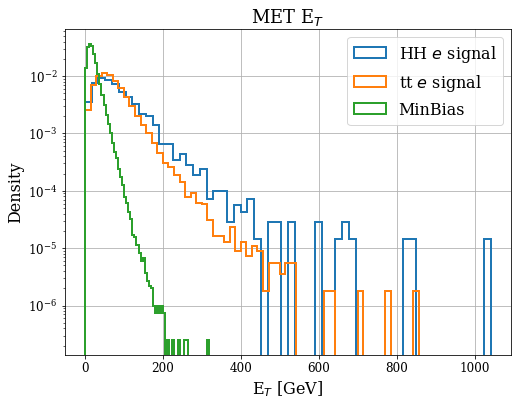
\includegraphics[width=0.66\linewidth]{Chapters/Plots/Hist_1ele_met_Et.png}
    %\vspace{4ex}
  \end{minipage} %%
  \begin{minipage}[b]{0.5\linewidth}
    \centering
    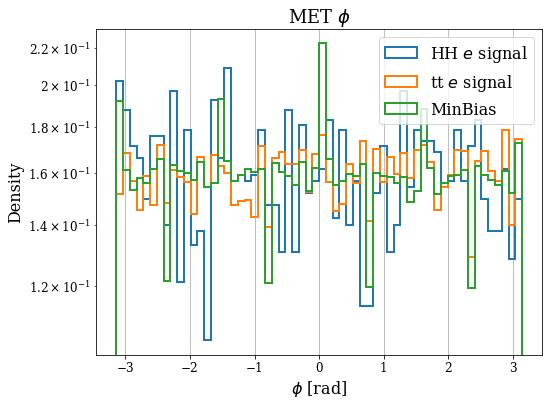
\includegraphics[width=0.66\linewidth]{Chapters/Plots/Hist_1ele_met_Phi.png}
    %\vspace{4ex}
  \end{minipage}
  \caption{Missing energy variables}
\end{figure}

\clearpage


\section{Input data set - muon channel -}
\begin{figure}[!ht] 
  \begin{minipage}[b]{0.33\linewidth}
    \centering
    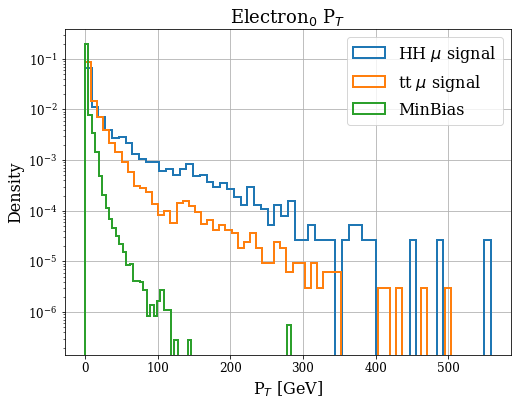
\includegraphics[width=1\linewidth]{Chapters/Plots/Hist_1mu_electron0_Et.png}
    %\vspace{4ex}
\end{minipage}%%
  \begin{minipage}[b]{0.33\linewidth}
    \centering
    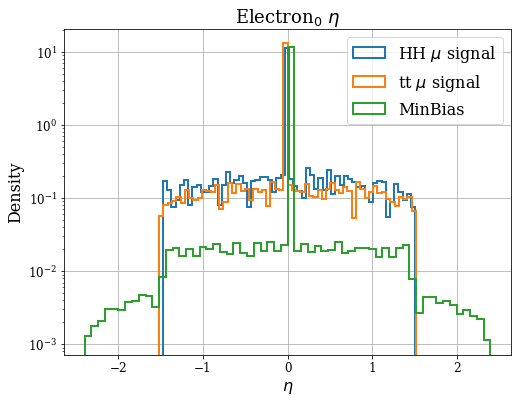
\includegraphics[width=1\linewidth]{Chapters/Plots/Hist_1mu_electron0_Eta.png}
    %\vspace{4ex}
\end{minipage} %%
  \begin{minipage}[b]{0.33\linewidth}
    \centering
    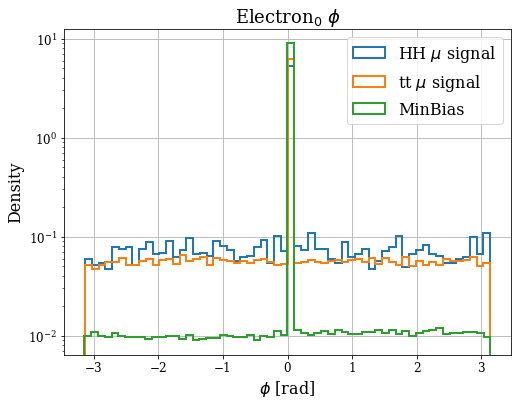
\includegraphics[width=1\linewidth]{Chapters/Plots/Hist_1mu_electron0_Phi.png}
    %\vspace{4ex}
  \end{minipage}
  \caption{Electron 0 variables}
\end{figure}


\begin{figure}[!ht] 
  \begin{minipage}[b]{0.33\linewidth}
    \centering
    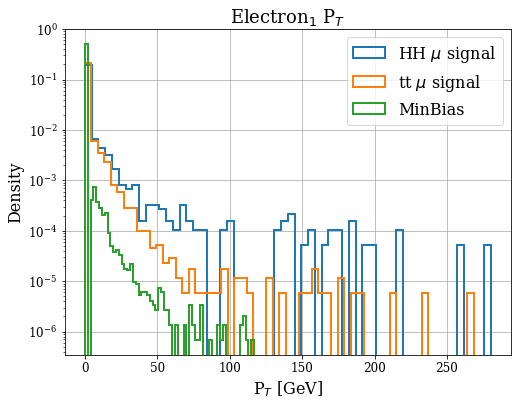
\includegraphics[width=1\linewidth]{Chapters/Plots/Hist_1mu_electron1_Et.png}
    %\vspace{4ex}
  \end{minipage}%%
  \begin{minipage}[b]{0.33\linewidth}
    \centering
    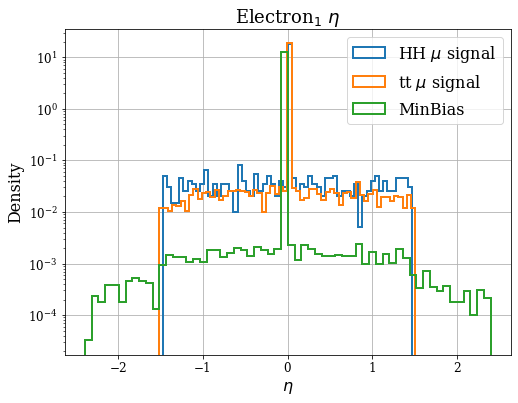
\includegraphics[width=1\linewidth]{Chapters/Plots/Hist_1mu_electron1_Eta.png}
    %\vspace{ex}
  \end{minipage} %%
  \begin{minipage}[b]{0.33\linewidth}
    \centering
    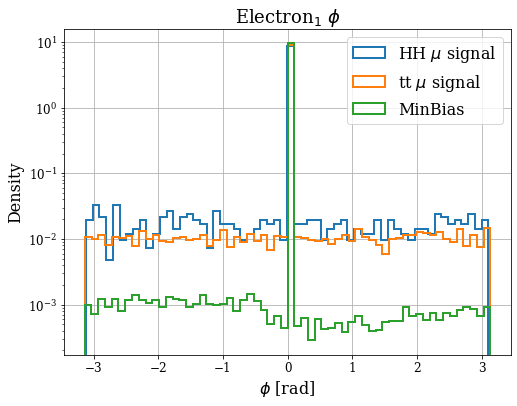
\includegraphics[width=1\linewidth]{Chapters/Plots/Hist_1mu_electron1_Phi.png}
    %\vspace{4ex}
  \end{minipage}
  \caption{Electron 1 variables}
\end{figure}


\begin{figure}[!ht]
  \begin{minipage}[b]{0.33\linewidth}
    \centering
    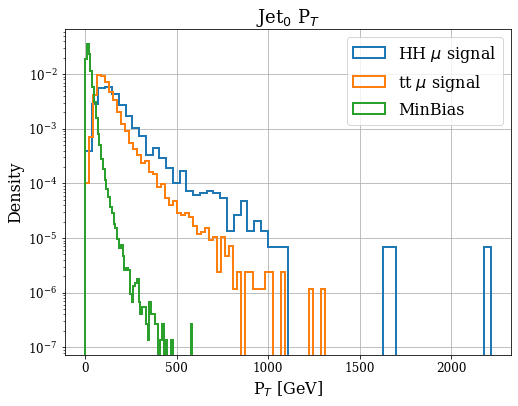
\includegraphics[width=1\linewidth]{Chapters/Plots/Hist_1mu_jet0_Et.png}
    %\vspace{4ex}
  \end{minipage}%%
  \begin{minipage}[b]{0.33\linewidth}
    \centering
    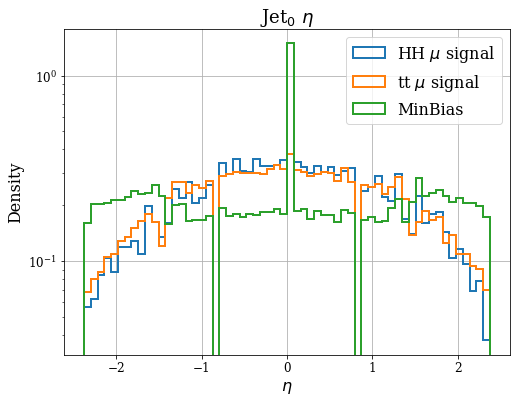
\includegraphics[width=1\linewidth]{Chapters/Plots/Hist_1mu_jet0_Eta.png}
    %\vspace{4ex}
  \end{minipage} %%
  \begin{minipage}[b]{0.33\linewidth}
    \centering
    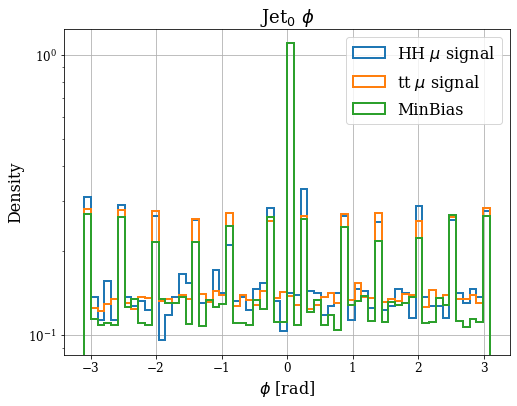
\includegraphics[width=1\linewidth]{Chapters/Plots/Hist_1mu_jet0_Phi.png}
    %\vspace{4ex}
  \end{minipage}
  \caption{Jet 0 variables}
\end{figure}

\begin{figure}[!ht]
  \begin{minipage}[b]{0.33\linewidth}
    \centering
    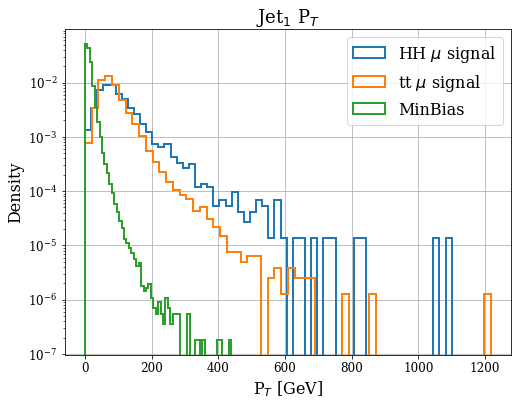
\includegraphics[width=1\linewidth]{Chapters/Plots/Hist_1mu_jet1_Et.png}
    %%%\vspace{4ex}
  \end{minipage}%%
  \begin{minipage}[b]{0.33\linewidth}
    \centering
    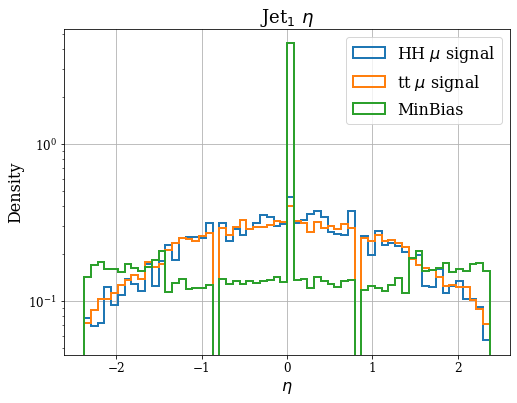
\includegraphics[width=1\linewidth]{Chapters/Plots/Hist_1mu_jet1_Eta.png}
    %%%\vspace{4ex}
  \end{minipage} %%
  \begin{minipage}[b]{0.33\linewidth}
    \centering
    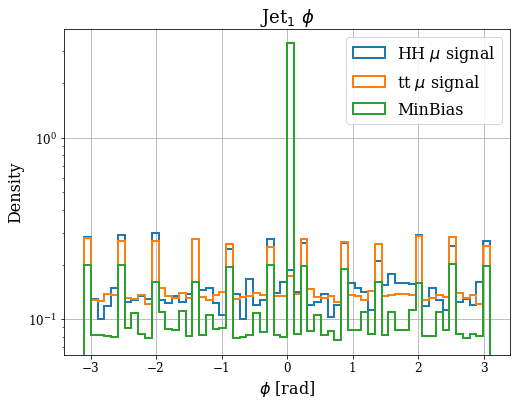
\includegraphics[width=1\linewidth]{Chapters/Plots/Hist_1mu_jet1_Phi.png}
    %%%\vspace{4ex}
  \end{minipage}
  \caption{Jet 1 variables}
 \end{figure}
 
 
 \begin{figure}[!ht]
  \begin{minipage}[b]{0.33\linewidth}
    \centering
    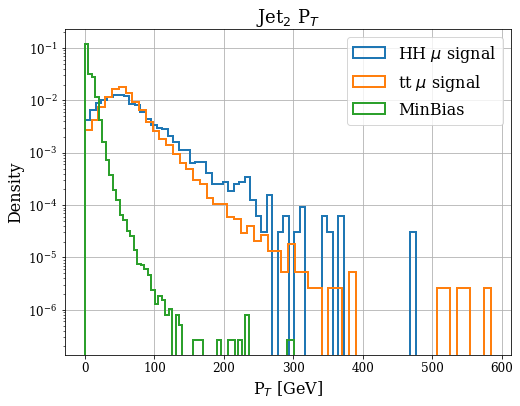
\includegraphics[width=1\linewidth]{Chapters/Plots/Hist_1mu_jet2_Et.png}
    %%%\vspace{4ex}
  \end{minipage}%%
  \begin{minipage}[b]{0.33\linewidth}
    \centering
    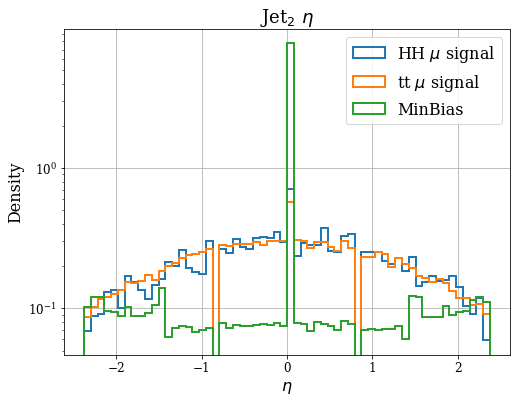
\includegraphics[width=1\linewidth]{Chapters/Plots/Hist_1mu_jet2_Eta.png}
    %%%\vspace{4ex}
  \end{minipage} %%
  \begin{minipage}[b]{0.33\linewidth}
    \centering
    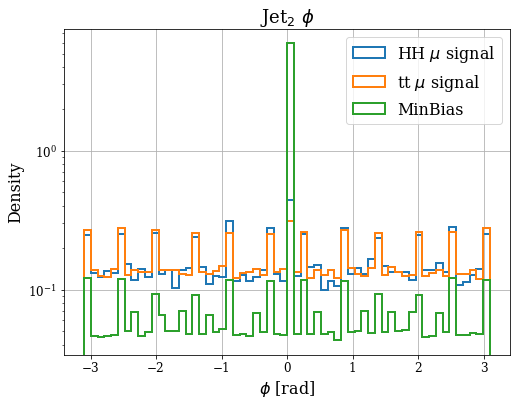
\includegraphics[width=1\linewidth]{Chapters/Plots/Hist_1mu_jet2_Phi.png}
    %%%\vspace{4ex}
  \end{minipage}
  \caption{Jet 2 variables}
\end{figure}


\begin{figure}[h]
  \begin{minipage}[b]{0.33\linewidth}
    \centering
    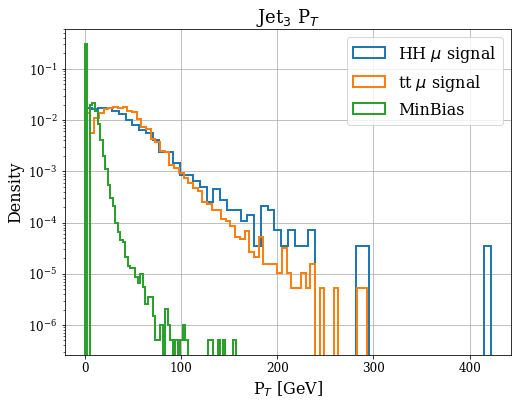
\includegraphics[width=1\linewidth]{Chapters/Plots/Hist_1mu_jet3_Et.png}
    %%%\vspace{4ex}
  \end{minipage}%%
  \begin{minipage}[b]{0.33\linewidth}
    \centering
    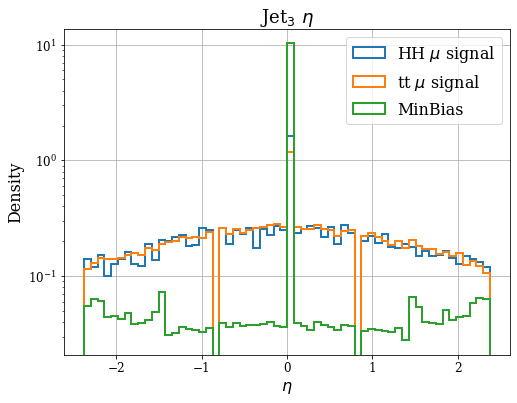
\includegraphics[width=1\linewidth]{Chapters/Plots/Hist_1mu_jet3_Eta.png}
    %%%\vspace{4ex}
  \end{minipage} %%
  \begin{minipage}[b]{0.33\linewidth}
    \centering
    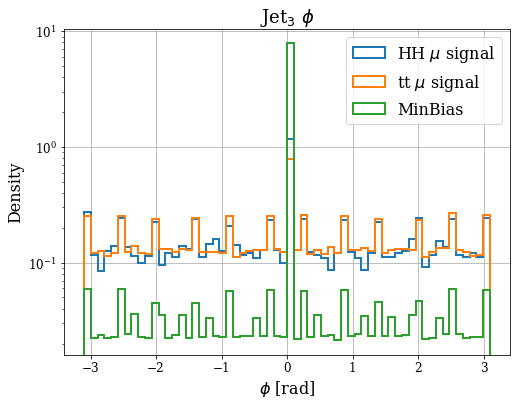
\includegraphics[width=1\linewidth]{Chapters/Plots/Hist_1mu_jet3_Phi.png}
    %%%\vspace{4ex}
  \end{minipage}
  \caption{Jet 3 variables}
\end{figure}


\begin{figure}[h]
  \begin{minipage}[b]{0.33\linewidth}
    \centering
    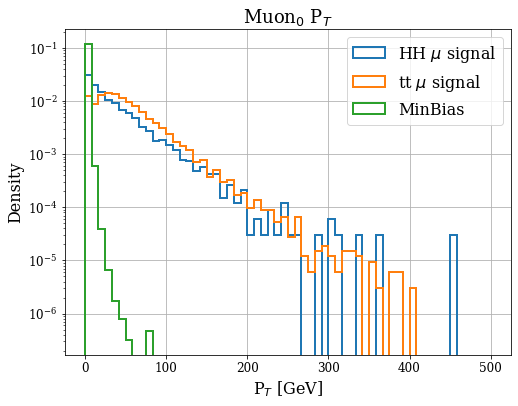
\includegraphics[width=1\linewidth]{Chapters/Plots/Hist_1mu_muon0_Pt.png}
    %%%\vspace{4ex}
  \end{minipage}%%
  \begin{minipage}[b]{0.33\linewidth}
    \centering
    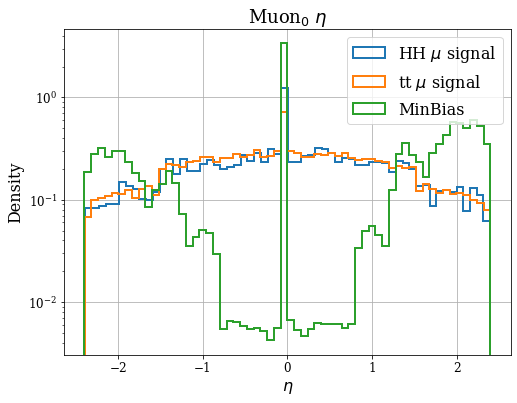
\includegraphics[width=1\linewidth]{Chapters/Plots/Hist_1mu_muon0_Eta.png}
    %%\vspace{4ex}
  \end{minipage} %%
  \begin{minipage}[b]{0.33\linewidth}
    \centering
    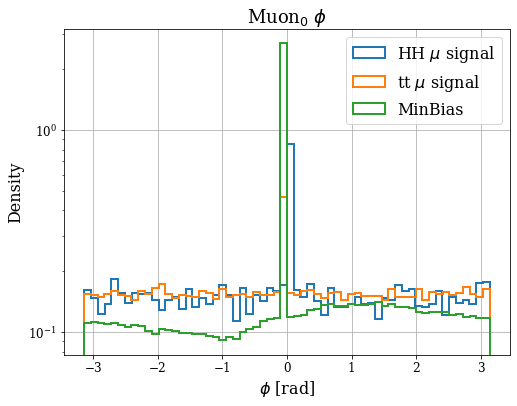
\includegraphics[width=1\linewidth]{Chapters/Plots/Hist_1mu_muon0_Phi.png}
    %%\vspace{4ex}
  \end{minipage}
  \caption{Muon 0 variables}
\end{figure}


\begin{figure}[h]
  \begin{minipage}[b]{0.33\linewidth}
    \centering
    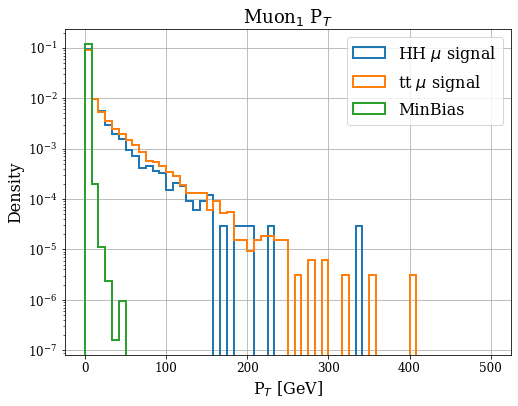
\includegraphics[width=1\linewidth]{Chapters/Plots/Hist_1mu_muon1_Pt.png}
    %%\vspace{4ex}
  \end{minipage}%%
  \begin{minipage}[b]{0.33\linewidth}
    \centering
    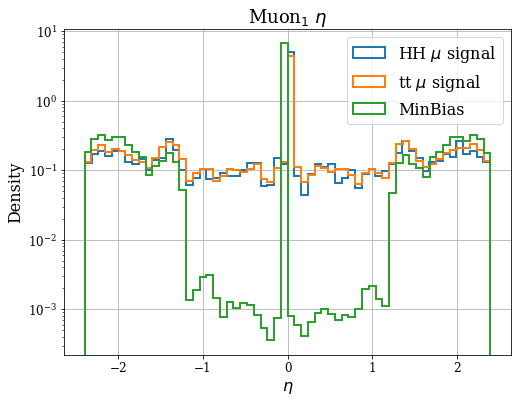
\includegraphics[width=1\linewidth]{Chapters/Plots/Hist_1mu_muon1_Eta.png}
    %\vspace{4ex}
  \end{minipage} %%
  \begin{minipage}[b]{0.33\linewidth}
    \centering
    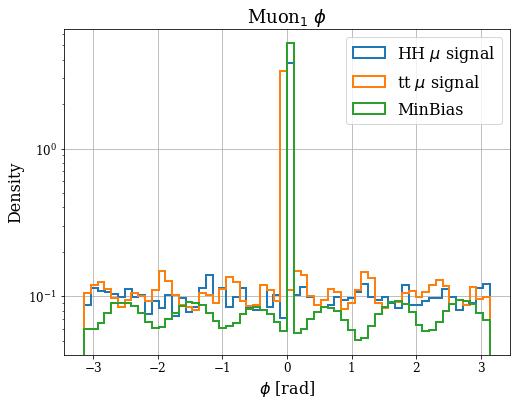
\includegraphics[width=1\linewidth]{Chapters/Plots/Hist_1mu_muon1_Phi.png}
    %\vspace{4ex}
  \end{minipage}
  \caption{Muon 1 variables}
\end{figure}


\begin{figure}[h]
  \begin{minipage}[b]{0.5\linewidth}
    \centering
    \includegraphics[width=0.66\linewidth]{Chapters/Plots/Hist_1mu_met_Et.png}
    %\vspace{4ex}
  \end{minipage} %%
  \begin{minipage}[b]{0.5\linewidth}
    \centering
    \includegraphics[width=0.66\linewidth]{Chapters/Plots/Hist_1mu_met_Phi.png}
    %\vspace{4ex}
  \end{minipage}
  \caption{Missing energy variables}
\end{figure}
\clearpage

    
\chapter{Design Implementation}
\label{sec:App_Desgin}

The Resource usage of the produced designs are given in table \ref{tab:Design-impl} alongside the the directives invoked during the synthesis and implementation steps in table \ref{tab:Design-directivesl}. The design of the GT-algo VU9P is the one used during the multi-board test with a small trigger menu of 24 algorithms. Each SLR contains the same 8 algorithms in table \ref{tab:test_algos}.
\begin{table}[h]
    \centering
    \begin{tabular}{c|c|c|c|c|c|c|c|c}
        GT-board & FPGA & LUT [\%] & FF [\%] & DSP [\%] & BRAM [\%] & URAM [\%] & Synth [h] & Impl [h] \\
        \hline
        GT-Algo   & VU9P  & 15.75 & 15.18 & 0.96 & 34.03 & 0 & 0.70 & 4.07  \\
        GT-Algo   & VU13P & - & - & - & - & - & - & -  \\
        GT-Finor  & VU9P  & 39.63 & 33.33 & 0 & 34.73 & 0 & 0.78 & 5.45  \\
        GF-Finor  & VU13P & 27.65 & 22.82 & 0 & 33.26 & 0 & 0.86 & 6.91  \\
    \end{tabular}
    \caption{Complete firmware resource usage}
    \label{tab:Design-impl}
\end{table}

\begin{table}[h]
    \centering
    \begin{tabular}{c|c|c}
        \multirow{2}{*}{GT-board} & \multicolumn{2}{c}{Directives} \\
        & Synth & Impl \\
        \hline
        \multirow{2}{*}{GT-Algo}    & flatten\_hierarchy none &  ExtraNetDelay\_high \\
           &  & AggressiveExplore  \\
        \hline
        \multirow{2}{*}{GT-Finor}  & flatten\_hierarchy=none & ExtraTimingOpt  \\
           &  AlternateRoutability & AlternateCLBRoutability \\
    \end{tabular}
    \caption{Synthesis and implementation directives}
    \label{tab:Design-directivesl}
\end{table}
    

\end{document}